% +------------------------------------------------------------------------+
% | CGAL Reference Manual:  snapRounding.tex
% +------------------------------------------------------------------------+
% | snap rounding of line segments
% |
% | 9.4.00   Eli Packer
% | 
\RCSdef{\snapRoundingRev}{$Revision$}
\RCSdefDate{\snapRoundingDate}{$Date$}
% +------------------------------------------------------------------------+

\ccParDims

% \usepackage{graphics, amssymb,epsfig}

\ccChapterRelease{\snapRoundingRev. \ \snapRoundingDate}\\
\ccChapterAuthor{Eli Packer}
\newcommand{\reals}{{\rm I\!\hspace{-0.025em} R}}
\def\A{{\cal A}}
\def\S{{\cal S}}

% +------------------------------------------------------------------------+
\section{Introduction}
Snap Rounding (SR, for short) is a well known method for converting
arbitrary-precision arrangements of segments into a fixed-precision
representation \cite{gght-srlse-97, gm-rad-98, h-psifp-99}. In
the study of robust geometric computing, it can be classified
as a finite precision approximation technique. Iterated Snap Rounding
(ISR, for short) is a modification of SR in which each vertex is at least
half-the-width-of-a-pixel away from any non-incident edge
\cite{cgal:hp-isr-02}. This package supports both methods. Algorithmic
details and experimental results are given in \cite{cgal:hp-isr-02}.

\begin{figure}
\begin{ccTexOnly}
\centerline{\includegraphics[width=10cm]{Snap_rounding_2/sr1.ps}}
\end{ccTexOnly}

\caption{An arrangement of segments before (a) and after (b)
SR (hot pixels are shaded)}
\label{fig:sr1}

\begin{ccHtmlOnly}
<P>
<center>
  <img src="sr1.gif"  border=0 alt="arrangement">
</center>
\end{ccHtmlOnly}
\end{figure}

\section{What is Snap Rounding/Iterated Snap Rounding}
Given a finite collection $\S$ of segments in the plane, the
arrangement of $\S$ denoted $\A(\S)$ is the subdivision of the plane
into vertices, edges, and faces induced by $\S$. %\cite{arrg-surveys}.
A {\it vertex\/} of the arrangement is either a segment endpoint or
the intersection of two segments. Given an arrangement of segments
whose vertices are represented with arbitrary-precision coordinates,
the SR procedure
(snap\_rounding\_2 $<$ traits,InputIterator,OutputContainer $>$)
proceeds as follows.  We tile the plane
with a grid of unit squares, {\it pixels}, each centered at a point
with integer coordinates. A pixel is {\it hot\/} if it contains a
vertex of the arrangement. Each vertex of the arrangement is replaced
by the center of the hot pixel containing it and each edge $e$ is
replaced by the polygonal chain through the centers of the hot pixels
met by $e$, in the same order as they are met by $e$. 
Figure~\ref{fig:sr1} demonstrates the results of SR.

In a snap-rounded arrangement, the distance between a vertex and
a non-incident edge can be extremely small compared with the width of a
pixel in the grid used for rounding. ISR
is a modification of SR which makes a vertex and a
non-incident edge well separated (the distance between each is at least
half-the-width-of-a-pixel). However, the guaranteed quality of the
approximation in ISR degrades. Figure~\ref{fig:isr_vs_sr} depicts
the results of SR and ISR on the same input.

\section{Terms and Software Design}

Our package supports both schemes, implementing the algorithm
described in \cite{cgal:hp-isr-02}.
Although the paper only describes an algorithm for ISR,
it is easy to derive an algorithm for SR, by performing only
the first rounding level for each segment.
%Theoretical bounds for the algorithm
%are $O(n\log n +I+L^{2/3}N^{2/3+\varepsilon}+L)$
%time for any $\varepsilon>0$ and $O(n+N+L^{2/3}N^{2/3+\varepsilon})$ working
%storage , where $I$ is the number of intersection points, $N$ is the number of
%hot pixels (which is at most $2n+I$) and $L$ is the overall number of links in
%the chains produced by the algorithm. The analysis assumes the use of
%partition trees as a search structure with which we answer segment/pixel
%intersection queries. Since it is difficult to implement, we used a data
%structure consisting of several kd-trees instead. Hence, the above bounds
%degrade but nor significantly.

There are three template parameters: \ccc{Traits} is the underlying geometry, i.e., the number type used
and the coordinate representation. \ccc{InputIterator} is the type of the iterators that point to the first
and after-the-last elements of the input. Finally, \ccc{OutputContainer} is the type of the output container.

Since the algorithm requires kernel functionalities such as the rounding to the center of a pixel, a special
traits class must be provided. The precise description of the requirements is given by the
concept SnapRoundingTraits\_2. The class Snap\_rounding\_traits\_2 is a model of this concept.

\begin{figure}
\begin{ccTexOnly}
\centerline{\includegraphics{Snap_rounding_2/isr_vs_sr.ps}}
\end{ccTexOnly}

\caption{An arrangement of segments before (a), after SR (b)
and ISR (c) (hot pixels are shaded).}
\label{fig:isr_vs_sr}

\begin{ccHtmlOnly}
<P>
<center>
  <img src="isr_vs_sr.gif"  border=0 alt="arrangement">
</center>
\end{ccHtmlOnly}
\end{figure}

%\psfig{figure=isr_vs_sr.ps,width=15cm} \

\section{Four Line Segment Example}

The following example generates an ISR representation
of an arrangement of four line segments
and a list of points which are the vertices of the resulting polylines.

\ccIncludeExampleCode{Snap_rounding_2/example.C}
% +--------------------------------------------------------+

% EOF
